\documentclass[10pt,conference,letterpaper]{IEEEtran}
\usepackage{amsmath,amssymb}
\usepackage{graphicx}
\usepackage{booktabs}
\usepackage{microtype}
\usepackage{url}
\graphicspath{{figures/}}
\setlength{\textfloatsep}{6pt plus 1pt minus 2pt}
\setlength{\floatsep}{6pt plus 1pt minus 2pt}

\title{Deterministic Target-Conditioned Gaussian-Process Optimization for Small-Budget Electromagnetic Design}
\author{\IEEEauthorblockN{Le Dong}
\IEEEauthorblockA{\textit{School of Electrical Engineering}\\
\textit{Xi'an Jiaotong University}\\
Xi'an, Shaanxi 710049, China\\
\texttt{leroi\_2024@stu.xjtu.edu.cn}}}

\begin{document}
\maketitle

\begin{abstract}
Electromagnetic component design often requires a target response within a strict tolerance band while minimizing a performance objective under a limited computational budget. To eliminate run-to-run variance under small evaluation budgets, we present a deterministic, target-conditioned Gaussian-process (GP) workflow that pairs center-point initialization and deterministic multi-start GP fitting with a two-stage feasibility-to-constrained-expected-improvement (cEI) search, adaptive relative-cEI stopping, and a final verification batch. With hyperparameters and stopping rules fixed on 14 development targets, the workflow recovers the exact global optimum on all 73 held-out targets of a 1,110-design air-core coil benchmark at an average cost of 21.81 evaluations per target. By contrast, six-point random initialization under the same fitting and stopping rules suffers from seed sensitivity, recovering 856 of 870 target–seed runs. When transferred without retuning to an eight-dimensional wireless-power-transfer (WPT) benchmark across 21 target mutual inductances, both the proposed workflow and budget-matched conventional cEI find feasible designs for all 21 targets, compared with 10/21 for quasirandom Sobol search. Relative to a fixed 50-evaluation budget, the adaptive stopping rule cuts evaluations by 30.3\% at the cost of a 3.79\% increase in mean DC resistance. Finally, in an 85-kHz 3-D Ansys Maxwell eddy-current verification at 1000 nH, the proposed workflow automatically terminates at 30 total evaluations with an AC resistance of $0.38368~\Omega$, outperforming a conventional cEI baseline matched to the same 30-evaluation budget ($0.38954~\Omega$).
\end{abstract}

\begin{IEEEkeywords}
Adaptive stopping, Bayesian optimization, constrained expected improvement, electromagnetic design, surrogate modeling.
\end{IEEEkeywords}

\section{Introduction}
Electromagnetic design frequently requires matching a target physical response within a strict tolerance band $\epsilon$ while minimizing a competing objective. For a forward model returning a constrained response $g(x)$ and scalar objective $J(x)$ ver design space $\mathcal X$, the target-conditioned optimization problem is
\begin{equation}
 \min_{x\in\mathcal X}J(x)\quad\mathrm{s.t.}\quad
 \frac{|g(x)-g_t|}{|g_t|}\leq\epsilon .
 \label{eq:problem}
\end{equation}
Here, $J(x)$ may represent winding resistance or a scalarized combination of loss, mass, thermal rise. Since each forward evaluation often requires an expensive finite-element simulation or hardware measurement, the total evaluation budget must remain small, while initial sampling, stochastic surrogate fitting, and stopping rules heavily influence the final design.

Gaussian-process Bayesian optimization (BO) is established in electromagnetic design. Online GP-assisted evolutionary search has been applied to antennas \cite{liu2014}, machine-learning-assisted antenna optimization has combined learned representations and GPs \cite{wu2024}, and BO has been used for WPT coil design \cite{sim2023}. Constrained expected improvement (cEI) is likewise established \cite{gardner}. Existing studies commonly report performance under fixed budgets, but initialization, GP-fit reproducibility, adaptive stopping, and final verification are rarely evaluated together under an explicit function-evaluation budget. We study how these choices affect a target-conditioned optimizer when only a small number of model evaluations is available.

This question connects three issues that are often reported separately. Initial-design size and placement can materially affect small-budget BO \cite{furuuchi2024}; random restarts in GP hyperparameter fitting can make identical data yield different numerical trajectories; and a fixed budget gives no task-dependent indication of when another model evaluation has little posterior value. Formal BO stopping criteria have been derived from posterior simple-regret reduction \cite{ishibashi2023}. Here, a simpler engineering threshold is fixed on development targets and tested against exhaustive optima on held-out targets.

The contributions are: 1) matched surrogate and acquisition studies for the coil benchmark; 2) a reproducible workflow that combines deterministic feasibility discovery and GP fitting with $B=N_0+N_{\rm seq}+N_{\rm ver}$ budget allocation and adaptive stopping; and 3) validation with 73 held-out exhaustive targets, 21 numerical WPT targets, and a matched-budget Maxwell case. The scope is observation-efficient and reproducible optimization on these electromagnetic models; no new acquisition function or general convergence result is claimed.

\section{Models and Optimization Method}
\subsection{Two-Dimensional Coil Model}
The first benchmark describes a multilayer air-core coil by radial layers $T\in\{1,\ldots,10\}$ and turns per layer $n\in\{20,\ldots,130\}$. With wire diameter $d=0.68$ mm, pitch $p=1.05d$, inner diameter $D_0=80$ mm, mean diameter $D=D_0+Tp$, height $H=np$, radial thickness $C=Tp$, total turns $N=Tn$, and resistivity $\rho=1.851\times10^{-5}\ \Omega\!\cdot\!\mathrm{mm}$, the analytical model is
\begin{equation}
 L=\frac{0.08N^2D^2\,10^{-4}}{3D+9H+10C}\ {\rm mH},\qquad
 R=\frac{4\rho ND}{d^2}.
 \label{eq:coil}
\end{equation}
The domain contains 1,110 integer designs. A design is feasible when $|L-L_t|/L_t\leq0.025$, and the objective is the smallest feasible $R$. Enumeration supplies an independent reference optimum for each target $L_t=1,\ldots,87$ mH. For a feasible returned design, bounded loss is $u=r/(1+r)$, where $r=R/R_{\rm exhaustive}-1$; infeasible returns have $u=1$.

\subsection{Reusable-Surrogate Screening}
Before target-specific optimization, we compare reusable dual-response GPs and ten-member neural ensembles under the same $B=17+10=27$ protocol: 17 globally reusable model-building observations and ten target-specific final evaluations. The random policies use 17 seeded uniform observations. Active policies begin with six of the same observations and acquire 11 more using equally weighted, scale-normalized uncertainty in $L$ and $R$. Every model family then uses the same final-ranking score and decision pool.

Fig.~\ref{fig:surrogates} shows that active selection improves both families, with the GP giving the stronger result under this budget. Random GP sampling finds feasible designs in 99.89\% of 870 cases and reaches 695 exact optima; active GP sampling finds feasible designs in every case, reaches 740 exact optima, and reduces all-case mean bounded loss from 0.00682 to 0.00287, a 57.9\% reduction. For the tested 16--8 ReLU ensemble, active sampling raises exact recovery from 274 to 651 and reduces mean loss from 0.310 to 0.104. The target-conditioned experiments therefore use GP surrogates.

\begin{figure}[!t]
 \centering
 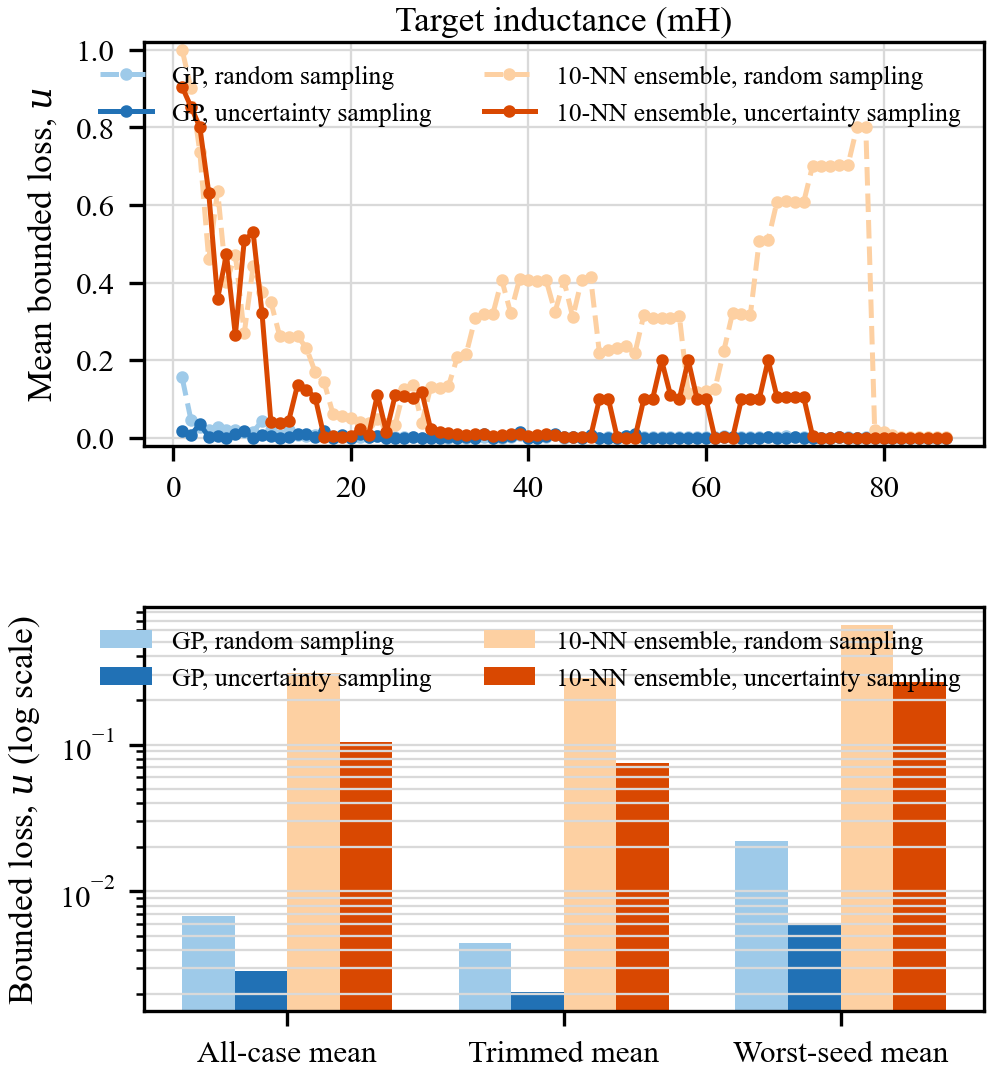
\includegraphics[width=0.90\columnwidth]{fig01_global_surrogate_2x2.png}
 \caption{Matched reusable-surrogate screen at nominal per-target $B=27$. Both model families use 17 shared model-building observations and the same ten target-specific final evaluations. Lower bounded loss is better.}
 \label{fig:surrogates}
\end{figure}

\subsection{Direct-Search Reference}
We also compare the selected reusable GP with simulated annealing (SA), which searches the integer domain directly using cached evaluations and stops after five cycles without a 1\% feasible-objective improvement \cite{kirkpatrick}. Both methods use the same $\pm2.5\%$ feasibility rule and the same ten seeds. Fig.~\ref{fig:gp-sa} shows trimmed mean bounded loss of 0.00205 for the GP and 0.0451 for SA, at 27 nominal evaluations versus 92.1. Moreover, the GP's 17 model-building observations are reused across all targets, whereas SA starts a separate search for every target. This result motivates the subsequent target-informed GP study.

\begin{figure}[!t]
 \centering
 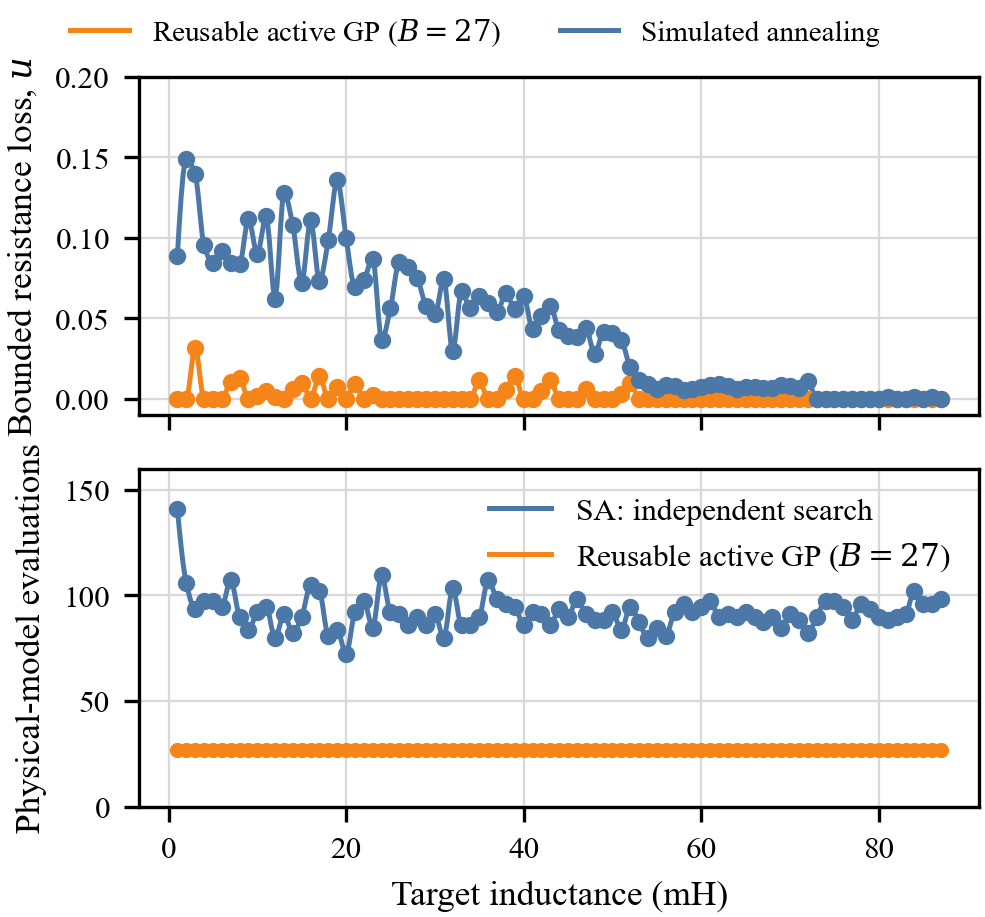
\includegraphics[width=0.90\columnwidth]{fig03_gaussian_process_vs_sa.png}
 \caption{Reusable active GP versus direct SA. The upper panel reports targetwise-trimmed bounded loss and the lower panel reports forward-model evaluations.}
 \label{fig:gp-sa}
\end{figure}

\subsection{Target-Conditioned Acquisition}
Independent GPs model $L$ and $R$ with radial-basis-function kernels and white-noise terms \cite{rasmussen}. For target $L_t$, the inductance GP gives
\begin{equation}
 p_F(x)=\Phi\!\left(\frac{L_t(1+\epsilon)-\mu_L}{\sigma_L}\right)
 -\Phi\!\left(\frac{L_t(1-\epsilon)-\mu_L}{\sigma_L}\right).
 \label{eq:pf}
\end{equation}
After a feasible observation exists, cEI maximizes $a_{\rm cEI}(x)=p_F(x)\mathrm{EI}_R(x)$. A matched $6+11+10=27$ comparison over ten seeds and 87 targets obtains 867/870 exhaustive optima with cEI, versus 829 for constrained lower confidence bound and 827 for integrated variance reduction. IVR nevertheless has much lower mean bounded loss than cLCB (0.000819 versus 0.00274), so their secondary ordering depends on the performance metric. cEI is strongest under both exact recovery and mean loss.

\subsection{Deterministic Feasibility Discovery and Fitting}
Before a feasible incumbent exists, maximizing $p_F$ alone can make a one-observation GP locally confident in the wrong region. We first observe the normalized domain center and then maximize
\begin{equation}
 a_F(x)=0.75\,\operatorname{norm}(p_F(x))
       +0.25\,\operatorname{norm}(\sigma_L(x)),
 \label{eq:start}
\end{equation}
where $\operatorname{norm}(\cdot)$ denotes candidate-wise min--max scaling. Once feasibility is found, selection switches to ordinary cEI. Kernel hyperparameters remain at their initial values for the first three observations. Thereafter, marginal likelihood is optimized from the initial point and four fixed Halton points in the bounded log-hyperparameter domain, and the best of these $K=5$ L-BFGS-B solutions is retained. Identical observations therefore yield identical fitted GPs.

Let $R_k^*$ be the best feasible resistance after refit $k$. We monitor maximum relative cEI
\begin{equation}
 \rho_k=\max_{x\in\mathcal C_k}
 \frac{p_F(x)\mathrm{EI}_R(x)}{R_k^*}.
 \label{eq:stop}
\end{equation}
The adaptive phase can stop only after at least $N_{\min}=2d+1$ model-building observations and after $\rho_k\leq0.01$ for three consecutive refits. It then evaluates ten verification candidates ranked by $p_F\exp[-\operatorname{norm}(\mu_R)]$; the returned design is the lowest-resistance feasible observation. The 1\% threshold is a termination measure based on posterior expected improvement over the searched candidates.

Each target follows five steps: (1) evaluate the domain center; (2) use (\ref{eq:start}) until a feasible observation is obtained; (3) refit both GPs from the fixed $K=5$ hyperparameter starts and acquire by cEI; (4) apply the minimum sample threshold and require three consecutive stopping-threshold hits; and (5) evaluate the final verification batch and return the best observed feasible design. Computational cost is measured by forward-model evaluations, with initialization, adaptive sampling, and verification reported separately.

\section{Experimental Protocol}
The 2-D targets are the 87 integers from 1 to 87 mH. Stochastic comparisons use ten fixed seeds, producing 870 target--seed cases. Every baseline receives the same model-evaluation budget and decision pool within its comparison. The acquisition study uses six initial observations, 11 sequential observations, and ten final evaluations. All losses and exact-recovery counts are recomputed against enumeration.

The feasibility weight is screened at ten targets spanning the domain. A separate 2--5 mH diagnostic examines the misses observed for random-six cEI. Stopping is developed on the union of these sets, giving 14 distinct targets. After fixing the 75/25 score, $K=5$, $\delta=1\%$, patience three, and ten verification evaluations, the remaining 73 targets are held out as a single final test. Replaying seed labels for the deterministic workflow verifies that the implementation is invariant to the unused seed input.

The numerical WPT study uses every 50-nH target from 1000 through 2000 nH. It compares the frozen workflow with six-Sobol-point conventional cEI, a center-start $p_F$-then-cEI control, Sobol search, and forced continuation. Conventional cEI receives the automatic run's realized targetwise budget. A separate 1000-nH Maxwell 3-D eddy-current test gives both policies 20 model-building and ten verification evaluations; the solver returns mutual inductance and the sum of the impedance matrix's Tx/Rx AC self-resistances at 85 kHz.

Raw records, hyperparameters, candidate histories, rendering scripts, and reproducibility checks accompany the manuscript. They verify budgets, losses, recovery totals, stopping histories, deterministic replay, and numerical and Maxwell WPT decisions. Each optimizer accesses the analytical equations through the same forward-model interface.

\section{Two-Dimensional Validation}
The feasibility weight, threshold, patience, and $K$ are selected on 14 development targets. All settings are then frozen and one deterministic trajectory is run at each of the remaining 73 targets. Every held-out run finds a feasible design and recovers the exhaustive optimum; all stop naturally. Mean total cost is 21.81 evaluations, median 22, and range 19--25. Model-building counts are 9--15, so the $2d+1=5$ minimum sample threshold is inactive for these trajectories; it protects against termination with insufficient data in higher-dimensional cases.

To separate deterministic fitting from starting-policy sensitivity, random-six initialization is also given the same 75/25 pre-feasibility score, fixed $K=5$ fitting, 1\% stopping rule, ten verification evaluations, and 27-evaluation ceiling. Across 870 seed--target cases it obtains 856 exact optima and seed-dependent decisions at eight targets. Pairing each random case with the deterministic result for the same target gives 14 deterministic wins, 856 ties, and no losses; mean costs are 22.57 and 21.93 evaluations.

At stopping, feasible-region posterior coverage on the 73 held-out tasks is 80.8\%/96.5\% at $1\sigma/2\sigma$ for $L$ and 82.1\%/96.3\% for $R$, whereas global coverage is substantially poorer. The pre-verification incumbent is already optimal in all 73 cases, so the final batch acts as a conservative verification allocation in this experiment.

Table~\ref{tab:two-d} separates the relevant comparisons. At $B=27$, cEI is the strongest tested target-conditioned acquisition under the uniform ten-evaluation final batch. The final comparison gives random and deterministic starts identical fitting and stopping criteria; the deterministic policy removes the remaining seed dependence.

\begin{table}[!t]
\caption{Summary of the 2-D evidence. Development and held-out rows have different denominators and are not pooled.}
\label{tab:two-d}
\centering
\scriptsize
\begin{tabular}{@{}lrrr@{}}
\toprule
Configuration & Cases & Exact & Mean evaluations \\
\midrule
cEI, fixed $6+11+10$ & 870 & 867 & 27.00 \\
Automatic, development & 14 & 14 & 22.571 \\
Automatic, held out & 73 & 73 & 21.808 \\
Random-six + same stopping & 870 & 856 & 22.570 \\
Deterministic center (unique) & 87 & 87 & 21.932 \\
\bottomrule
\end{tabular}
\end{table}

\begin{figure}[!t]
 \centering
 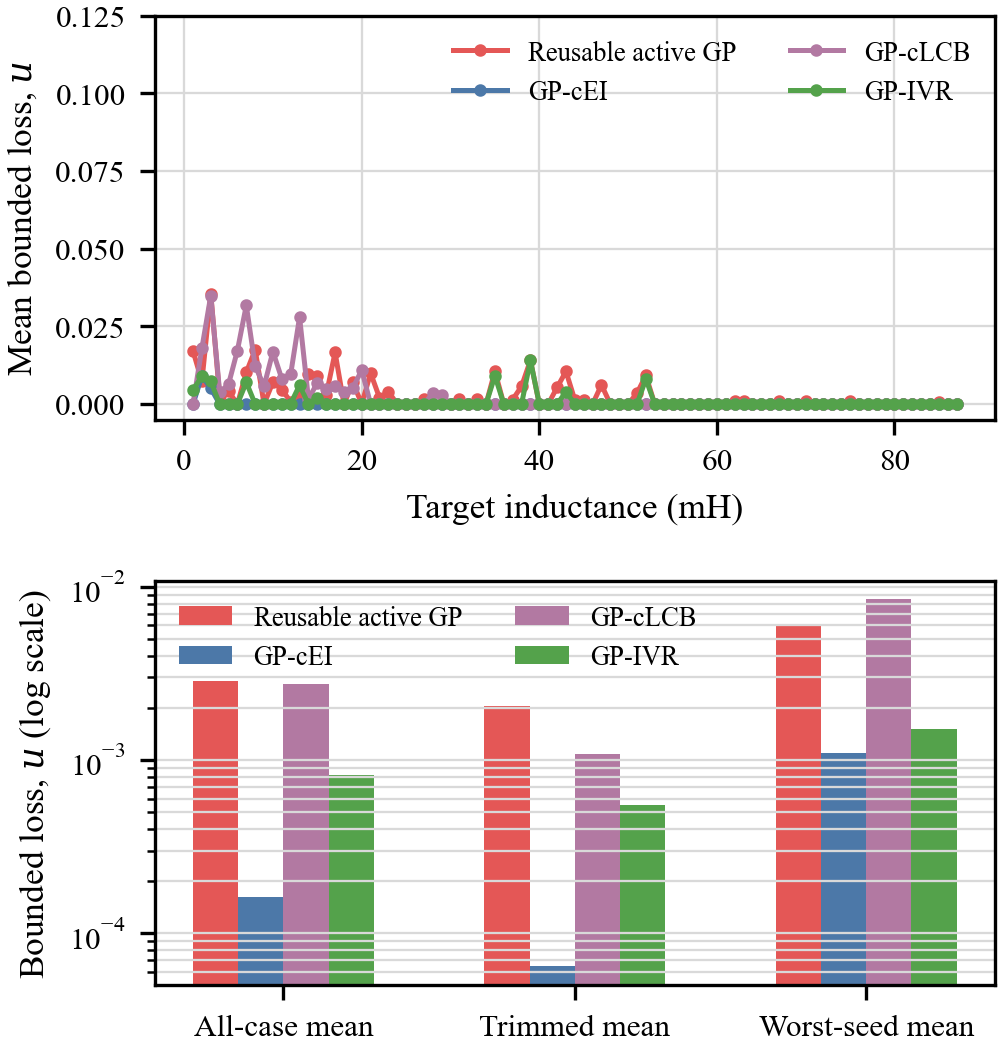
\includegraphics[width=0.98\columnwidth]{fig04_gp_acquisition_comparison.png}
 \caption{Matched target-conditioned acquisition comparison at $B=27$ over ten seeds and 87 targets. Lower bounded loss is better.}
 \label{fig:acquisition}
\end{figure}

\begin{figure*}[!t]
 \centering
 \includegraphics[width=0.90\textwidth]{fig05_automated_stopping.png}
 \caption{Automatic budgeting. (a) Mean total evaluations on the 14-target development screen; every configuration reaches the exhaustive optimum. (b) Model-building trace for the representative 1500-nH WPT case. (c) Maximum relative cEI after feasibility; three consecutive values below 1\% trigger stopping, followed by ten verification evaluations.}
 \label{fig:stopping}
\end{figure*}

\section{Application to Eight-Dimensional WPT Coil Design}
\subsection{Controlled Black-Box Benchmark}
The source WPT model has eight intrinsic geometry variables and six pose variables \cite{asadi2025}. We optimize the eight geometry variables: polygon side count $n_s\in[4,10]$, turn count $n_t\in[5,15]$, spacing $s\in[1,3]$ mm, and inner radius $r_i\in[30,80]$ mm for each transmitter and receiver. The counts are integral; $s$ and $r_i$ are continuous. Translation is fixed at $(0,0,70)$ mm and rotations are zero.

The constraint is $|M(x)-M_t|/M_t\leq0.025$. Total DC resistance is computed from polygonal conductor centerline length,
\begin{equation}
 R=\frac{\rho_{\rm Cu}}{A}\sum_{q\in\{t,r\}}\sum_{k=0}^{n_{t,q}-1}
 2n_{s,q}r_{q,k}\sin(\pi/n_{s,q}),
 \label{eq:wpt-r}
\end{equation}
where $r_{q,k}=r_{i,q}+k(s_q+w)$, $w=0.68$ mm, $A=\pi(w/2)^2$, and $\rho_{\rm Cu}=1.851\times10^{-5}\ \Omega\!\cdot\!\mathrm{mm}$. Leads are excluded. Mutual inductance is computed using the partial-inductance model in \cite{asadi2025}.

Both responses are presented to the optimizer as black-box outputs and learned by separate GPs. This provides a controlled comparison under equal evaluation budgets; the subsequent Maxwell experiment tests direct operation with a field solver.

The normalized center is evaluated first. Consecutive blocks of one unscrambled Sobol sequence provide deterministic candidates. Isotropic Mat\'ern-$5/2$ GPs use the same fixed $K=5$ fitting, 75/25 feasibility rule, 1\% stopping threshold, patience three, and ten verification evaluations. With $d=8$, $N_{\min}=17$; at most 40 model-building evaluations plus ten verification evaluations are allowed. No setting is retuned after the 2-D study.

\subsection{Results}
Across the 21 targets, automatic and conventional cEI both find feasible designs in 21/21 cases, versus 10/21 for Sobol. Their mean resistances are $0.31500$ and $0.31549\ \Omega$; wins/ties/losses are 8/3/10, with paired Wilcoxon $p=0.913$. Four trajectories stop at the $2d+1=17$ minimum sample threshold.

\begin{table}[!t]
\caption{Eight-dimensional WPT benchmark. $B_s$ and $R_s$ are the automatic stopping cost and resistance; $R_{50}$ is its forced-50 continuation. Five representative targets precede the full aggregate. Dashes indicate that no feasible design was found at the matched budget.}
\label{tab:wpt}
\centering
\scriptsize
\begin{tabular}{@{}rrrrrr@{}}
\toprule
$M_t$ (nH) & $B_s$ & $R_s$ & $R_{50}$ & Conv. & Sobol \\
& & \multicolumn{4}{c}{Resistance (m$\Omega$)} \\
\midrule
1000 & 33 & 259.7 & 259.7 & 259.7 & -- \\
1250 & 34 & 291.5 & 280.3 & 340.4 & -- \\
1500 & 44 & 305.8 & 305.8 & 305.6 & 343.9 \\
1750 & 27 & 332.5 & 324.9 & 332.5 & -- \\
2000 & 27 & 377.0 & 343.7 & 371.1 & 422.8 \\
\midrule
Mean (21) & 34.86 & 315.0 & 303.5 & 315.5 & -- \\
Feasible & -- & 21/21 & 21/21 & 21/21 & 10/21 \\
\bottomrule
\end{tabular}
\end{table}

Twenty runs stop naturally; 1150 nH reaches the 40-evaluation cap. Compared with forced $B=50$, stopping uses 30.3\% fewer evaluations with 3.79\% higher mean resistance. At 1500 nH, $M=1466.48$ nH and $R=0.30577\ \Omega$, leaving a 3.98-nH margin above the lower feasibility bound.

\subsection{Field-Solver Application Check}
At 1000 nH, the frozen automatic workflow stops after 20 model-building evaluations and then performs ten fixed verification evaluations. A matched baseline uses six fixed Sobol points, 14 conventional-cEI evaluations, and ten verification evaluations. Both find feasible designs. The automatic run yields seven feasible observations, $M=998.929$ nH, and $R_{\rm AC,Tx}+R_{\rm AC,Rx}=0.383681\ \Omega$; the baseline yields three, $1016.402$ nH, and $0.389535\ \Omega$. The automatic objective is 1.50\% lower, while the baseline reaches feasibility earlier (evaluation 6 versus 12). A common mesh-convergence study is required to resolve this small resistance difference.

In the numerical 1500-nH example, Tx/Rx use 9/7 sides, 7/7 turns, 1.741/2.709-mm spacing, and 61.724/61.007-mm inner radii. Feasibility occurs at model evaluation 12; stopping at 34 plus ten verification evaluations gives $B=44$, and forced continuation returns the same design.

\begin{figure}[!t]
 \centering
 \includegraphics[width=0.82\columnwidth]{fig06_wpt_selected_geometry.png}
 \caption{Selected nominal-pose 1500-nH design. The aligned transmitter and receiver planes are separated by 70 mm.}
 \label{fig:wpt-geometry}
\end{figure}

\section{Discussion and Conclusion}
The experiments support a compact engineering procedure: begin at the domain center, combine predicted feasibility with constraint uncertainty until a feasible observation exists, fit each GP from fixed low-discrepancy hyperparameter starts, require at least $2d+1$ observations, and terminate after persistently low relative cEI before evaluating a final verification batch. This removes implementation-level seed variation and performs consistently across the complete 2-D target lattice. On the WPT benchmark, its principal benefit is reliable feasibility with an adaptive evaluation budget.

The 75/25 feasibility score and stopping threshold are empirical settings established on the development set. The 2-D study uses an analytical model, the numerical WPT study fixes the relative pose, and the Maxwell comparison contains one trajectory per policy; experimental hardware validation and broader high-fidelity studies remain future work. Code, data, and validation scripts are available at \url{https://github.com/le-dong-xjtu/reproducible-target-informed-gp}.

\begin{thebibliography}{00}
\bibitem{rasmussen} C. E. Rasmussen and C. K. I. Williams, \emph{Gaussian Processes for Machine Learning}. MIT Press, 2006.
\bibitem{gardner} J. Gardner, M. Kusner, Z. Xu, K. Weinberger, and J. Cunningham, ``Bayesian optimization with inequality constraints,'' in \emph{Proc. ICML}, vol. 32, 2014, pp. 937--945.
\bibitem{liu2014} B. Liu \emph{et al.}, ``An efficient method for antenna design optimization based on evolutionary computation and machine learning techniques,'' \emph{IEEE Trans. Antennas Propag.}, vol. 62, no. 1, pp. 7--18, 2014.
\bibitem{wu2024} Q. Wu, W. Chen, C. Yu, H. Wang, and W. Hong, ``Machine-learning-assisted optimization for antenna geometry design,'' \emph{IEEE Trans. Antennas Propag.}, vol. 72, no. 3, pp. 2083--2095, 2024.
\bibitem{sim2023} B. Sim \emph{et al.}, ``Bayesian optimization based fast and accurate wireless power transfer system coil optimization for high efficiency,'' in \emph{Proc. IEEE WPTCE}, 2023.
\bibitem{asadi2025} M. Asadi and A. M. Abazari, ``A data-driven model to predict mutual inductance between planar coils with arbitrary specifications and positions,'' \emph{IET Electr. Power Appl.}, vol. 19, Art. no. e70015, 2025.
\bibitem{furuuchi2024} S. Furuuchi and S. Yamada, ``Verifying the effect of initial sample size in Bayesian optimization,'' \emph{Total Quality Science}, vol. 10, no. 1, pp. 8--19, 2024.
\bibitem{ishibashi2023} H. Ishibashi, M. Karasuyama, I. Takeuchi, and H. Hino, ``A stopping criterion for Bayesian optimization by the gap of expected minimum simple regrets,'' in \emph{Proc. AISTATS}, vol. 206, 2023, pp. 6463--6497.
\bibitem{kirkpatrick} S. Kirkpatrick, C. D. Gelatt, Jr., and M. P. Vecchi, ``Optimization by simulated annealing,'' \emph{Science}, vol. 220, no. 4598, pp. 671--680, 1983.
\end{thebibliography}

\end{document}
